\begin{ledgroupsized}[r]{120mm}
\footnotesize
\pstart
\noindent\textbf{Überlieferung:}
\pend
\end{ledgroupsized}
\begin{ledgroupsized}[r]{114mm}
\footnotesize
\pstart \parindent -6mm
\makebox[6mm][l]{\textit{L}}%
Konzept:
LBr~724 Bl.~18\textendash19. %
Ein Bogen~2\textsuperscript{o}.
{Wasserzeichen} in Bl.~18 und 
{Gegenmarke} in Bl.~19.
Vier Seiten.
Der Text ist vorwiegend linksspaltig geschrieben, aber die zahlreichen Änderungen und Ergänzungen (bes.\ im mittleren Textabschnitt, 18~v\textsuperscript{o}\textendash19~r\textsuperscript{o}) bedingen Sprünge in der Textfolge. %
Am Rand von 19~v\textsuperscript{o}, gegenläufig zum Text, eigh.\ Vermerk \glqq\textit{Pfautz}\grqq; der Bogen ist im Pfautz-Briefwechsel (LBr~724) überliefert. 
\pend
\end{ledgroupsized}
\selectlanguage{latin}
\vspace{8mm}
\pstart%
\noindent%
\href{\Scan{LBr_724_18r}}%
{\lbrack18~r\textsuperscript{o}\rbrack}
\lbrack%
\textit{Nachfolgend kleingedruckter Text (erste Fassung von \refpassage{LBr_724_018-019_13a}{LBr_724_018-019_13b}) gestrichen:}\rbrack %
\pend
\vspace{0.5em}
\footnotesize
\pstart 
\noindent
\edlabel{LBr_724_018-019_8a}%
\edtext{}{%
\xxref{LBr_724_018-019_8a}{LBr_724_018-019_8b}%
\lemma{Intelligo \lbrack...\rbrack\ pondera}%
\Cfootnote{%
Leibniz übernimmt in beträchtlichem Maße den Wortlaut 
von \indexN{\textls{Vanni}, Giovanni Francesco 1638\textendash1709}Vannis
\cite{02010}Brief an 
\indexN{\textls{Magliabechi} (Magliabecchi, Magliabecki, Magliabekius, Magliabequius), Antonio 1633\textendash1714}Magliabechi 
vom 5. Juni 1685,
den Leibniz über \indexN{\textls{Pfautz} (Pfauzius), Christoph 1645\textendash1711}C.~Pfautz
bekommen (siehe \cite{02009}\textit{LSB} III, 4 N.\;96) und abgeschrieben hatte (ebd. \cite{02010}N.\;97, hier S.\;222).}}%
\edtext{Intelligo 
\indexN{\textls{Vanni}, Giovanni Francesco 1638\textendash1709}autorem 
\cite{01995}\textit{Speciminis libri de momentis gravium}}{%
\lemma{}%
\Afootnote{\textit{Am Rand, nicht gestrichen:} %
\indexN{\textls{Vanni}, Giovanni Francesco 1638\textendash1709}
I.\,F.\,V. Lucensis\textsuperscript{\lbrack a\rbrack} viro\textsuperscript{\lbrack b\rbrack}
\lbrack\textit{Text bricht ab.}\rbrack\
\\[1.5ex]%
{\footnotesize%
\textsuperscript{\lbrack a\rbrack} Lucensis\ %
\textit{(1)}~Epistola %
\textit{(2)}~viro \textit{L}\quad
\textsuperscript{\lbrack b\rbrack} I.\,F.\,V. Lucensis viro: Abbrechende Abschrift der Eingangsformel in
\indexN{\textls{Vanni}, Giovanni Francesco 1638\textendash1709}Vannis
\cite{02010}Brief an 
\indexN{\textls{Magliabechi} (Magliabecchi, Magliabecki, Magliabekius, Magliabequius), Antonio 1633\textendash1714}A.~Magliabechi 
vom 5. Juni 1685, der Vorlage für die Textpassage \refpassage{LBr_724_018-019_8a}{LBr_724_018-019_8b} war: \glqq I.\,F.\,V. Lucensis Viro Ill\textsuperscript{mo} Antonio Magliabechio Ser\textsuperscript{mi} M.\;D. Etruriae Bibliothecae praefecto S.\;P.\grqq.}}}
in \cite{01023}\textit{Actis eruditorum} mensis Novemb. 1684.
\edtext{cum animadversione}{%
\lemma{cum}%
\Bfootnote{%
\textit{(1)}~animadversione %
\textit{(2)}~annotatione %
\textit{(3)}~animadversione~\textit{L}}}
quadam recusi, respondisse, primum ab 
\indexN{\textls{Leibniz} (Leibnitius, GGL), Gottfried Wilhelm 1646\textendash1716}autore 
\edtext{animadversionis in ea quam objecit \textls{instantia} perverti \cite{01995}\textit{Speciminis} Hypothesin;}{%
\lemma{animadversionis}%
\Bfootnote{%
\bars{autore \textit{gestr.}} %
\textit{(1)}~perverti suam %
\textit{(2)}~in ea quam objecit \textls{instantia} perverti \textit{Speciminis} Hypothesin;~\textit{L}}}
\edlabel{LBr_724_018-019_1a}%
\edtext{}{%
\xxref{LBr_724_018-019_1a}{LBr_724_018-019_1b}%
\lemma{}%
\Afootnote{%
\textit{Am Rand, gestrichen:} %
{\footnotesize Man kan die andere figur pag.~512. vorigen jahres, und die Figur p.~514. wieder hiehehr transferiren\textsuperscript{\lbrack a\rbrack}
\\[1.5ex]%
\textsuperscript{\lbrack a\rbrack} 
Gemeint sind die Figuren in \textsc{Vanni}\indexN{\textls{Vanni}, Giovanni Francesco 1638\textendash1709}, \cite{01995}\textit{Specimen libri de momentis gravium},
\cite{01023}\textit{AE} November 1684, S.\;512 und in Leibnizens Begleittext (N.\;\ref{55606}), ebd. S.\;514.
Siehe N.\;\ref{55606} mit den Diagrammen \lbrack\textit{Fig.~1}\rbrack\ und \lbrack\textit{Fig.~2}\rbrack\ auf S.~\pageref{Fig:AE_1684_514_fig-1-2}
sowie hier \lbrack\textit{Fig.~3}\rbrack\ auf S.~\pageref{Fig:LBr_724_018-019_fig-3}.}}}%
angulum enim duorum planorum\indexS{planum inclinatum}\indexS{angulus duorum planorum ad se invicem}
\textit{XC} et \textit{ZC} ad se invicem debere esse rectum, alioqui non
applicarentur globo\indexS{globus} in 
\edtext{\lbrack lineis\rbrack}{%
\lemma{}%
\Bfootnote{%
planis 
\textit{L ändert Hrsg.}}}
directionis,\indexS{linea directionis} in quo demonstrationis nervus
\edtext{consistat, \indexN{\textls{Leibniz} (Leibnitius, GGL), Gottfried Wilhelm 1646\textendash1716}%
animadversorem vero unum}{%
\lemma{consistat,}%
\Bfootnote{%
\textit{(1)}~autorem vero animadversionis unum %
\textit{(2)}~animadversorem vero unum~\textit{L}}}
ex planis fecisse verticale\indexS{planum verticale} alterum
\edtext{declive.\indexS{planum declive}\edlabel{LBr_724_018-019_1b} Deinde 
\indexN{\textls{Leibniz} (Leibnitius, GGL), Gottfried Wilhelm 1646\textendash1716}animadversorem}{%
\lemma{declive.}%
\Bfootnote{%
\textit{(1)}~Eundem autorem %
\textit{(2)}~Deinde %
\textit{(a)}~autorem animadversionis %
\textit{(b)}~animadversorem~\textit{L}}}
demonstrationi ipsi \cite{01995}\textit{Speciminis} frustra satisfacere conari, negando duo
\edtext{momenta\indexS{momentum in plano declivi} in planis declivibus\indexS{plana declivia angulum rectum facientia} facientibus angulum}{%
\lemma{momenta}%
\Bfootnote{%
\textit{(1)}~in duobus planis diversis %
\textit{(a)}~componere %
\textit{(b)}~cui
\textit{(c)}~quibus grave simul incumbit, componere momentum %
\textit{(d)}~quibus grave %
\textit{(2)}~in planis declivibus facientibus 
\textit{(a)}~in
\textit{(b)}~angulum~\textit{L}}}
rectum in unum posse addi,\indexS{additio momentorum} nam evidens
esse momenta\indexS{momentum} in unum posse addi,\indexS{additio momentorum} ut pondera.%
\edlabel{LBr_724_018-019_8b}		%
\pend
\normalsize
\begin{edfigure}%
\hfill
\includegraphics[scale=1]{%
gesamttex/edit_VIII-4/images/LBr_724_018-019_d1_018r.pdf}
\hfill
\includegraphics[scale=1]{%
gesamttex/edit_VIII-4/images/LBr_724_018-019_d2_018r.pdf}
\hfill
\edcaption{%
\hspace*{7mm}%
\edtext{\lbrack\textit{Fig.~1, nicht gestr.}\rbrack}{%
\lemma{\lbrack\textit{Fig.~1}\rbrack}%
\Cfootnote[nonum]{Ein gestrichener Entwurf zum Diagramm wird nicht wiedergegeben.}}%
\hspace*{18mm}%
\lbrack\textit{Fig.~2, nicht gestr.}\rbrack}
\end{edfigure}
\footnotesize
\pstart
Ad hanc responsionem ita replicari
posse visum est:
\edtext{primum in animadversione non perverti \cite{01995}\textit{Speciminis} hypothesin,}{%
\lemma{primum}%
\Bfootnote{%
\textit{(1)}~autorem %
\textit{(2)}~in animadversione non perverti %
\textit{(a)}~autoris h %
\textit{(b)}~\textit{Speciminis} hypothesin,~\textit{L}}}
sed aliam in ejus locum substitui, in qua facilius apparet
modum concludendi \cite{01995}\textit{Speciminis} non procedere. Quanquam 
autem
\edtext{recte notetur in responsione magnum}{%
\lemma{recte}%
\Bfootnote{%
\textit{(1)}~notet aut %
\textit{(2)}~notetur in responsione, %
\textit{(a)}~cum angulus planorum non est rectus %
\textit{(b)}~magnum~\textit{L}}}
esse discrimen inter casum anguli planorum recti\indexS{angulus planorum rectus} et acuti\indexS{angulus planorum acutus}\lbrack,\rbrack\ attamen
secundum ipsius argumentandi modum, cum 
\lbrack\textit{Text bricht ab.}\rbrack
\pend
\normalsize %
\vspace{0.5em} %
\pstart
\noindent
\lbrack%
\textit{Nachfolgend kleingedruckter Text (zweite Fassung von \refpassage{LBr_724_018-019_13a}{LBr_724_018-019_13b}) in \textit{L} teilweise gestrichen:}\rbrack%
\pend
\vspace{0.5em}
\footnotesize
\pstart
\noindent
Ad animadversionem in \cite{01023}\textit{Actis}
Novemb. 1684.\
\edtext{p.~514.\ \indexN{\textls{Vanni}, Giovanni Francesco 1638\textendash1709}autor 
\cite{01995}\textit{Speciminis} respondit}{%
\lemma{p.~514.}%
\Bfootnote{%
\textit{(1)}~respondet autor %
\textit{(a)}~momenti %
\textit{(b)}~\textit{Speciminis}, ut %
\textit{(2)}~autor \textit{Speciminis} respondit~\textit{L}}}
\textls{1\textsuperscript{\textls{mo}} ad instantiam,} in ea angulum planorum\indexS{angulus planorum} non
esse rectum, et ideo non posse momenta\indexS{momentum} in unum
\edtext{addi.\indexS{additio momentorum} Qua quidem responsione, autoris sententia ita declaratur,}{%
\lemma{addi.}%
\Bfootnote{%
\textit{(1)}~Quae quidem responsio bona %
\textit{(a)}~videtur, %
\textit{(b)}~est, %
\textit{(aa)}~autor %
\textit{(bb)}~objectio autem ex %
\textit{(aaa)}~ea o %
\textit{(bbb)}~eo orta erat, quod 
\textit{(aaaa)}~autor \textit{Speciminis},
\textit{(bbbb)}~\textit{Specimen}, in sua ratiocinatione, %
\textit{(ccc)}~ex eo quod dixisset %
\textit{(aaaa)}~glo %
\textit{(bbbb)}~planum quod totaliter descensum impedit, ut %
\textit{(2)}~Et quidem fatenda est ratio disparitatis %
\textit{(3)}~Et sane fatenda est disparitas %
\textit{(4)}~Et si \bars{quidem \textit{erg.}} autoris senten %
\textit{(5)}~Hinc apparet autoris sententia
\textit{(6)}~Qua quidem responsione %
\textit{(a)}~, intellecta sic autoris %
\textit{(aa)}~hypothesi, ut %
\textit{(bb)}~sententia, %
\textit{(b)}~autoris sententia ita declaratur,~\textit{L}}}
ut additio momentorum\indexS{additio momentorum} ipsi tantum locum habeat, cum plana
\edtext{faciunt angulum}{%
\lemma{faciunt}%
\Bfootnote{%
\textit{(1)}~ad %
\textit{(2)}~angulum~\textit{L}}}
rectum,\indexS{plana declivia angulum rectum facientia}
\edtext{ac proinde}{%
\lemma{}%
\Bfootnote{%
ac proinde %
\textit{erg.~L}}}
videtur instantiae satisfactum\lbrack,\rbrack\
\edlabel{LBr_724_018-019_6a}%
\edtext{}{%
\xxref{LBr_724_018-019_6a}{LBr_724_018-019_6b}%
\lemma{quae tamen}%
\Bfootnote{%
\textit{(1)}~non %
\textit{(2)}~vel ideo non sine ratione objecta fuit, quia %
\textit{(a)}~verum semper est %
\textit{(b)}~quemcunque angulum faciant plana inter se, tamen %
\textit{(aa)}~vim %
\textit{(bb)}~eodem jure \lbrack...\rbrack\ aequalia %
\textit{(aaa)}~sunt %
\textit{(bbb)}~esse \bars{semper \textit{gestr.}} momento %
\textit{(aaaa)}~quo pr %
\textit{(bbbb)}~totali. Sed %
\textit{erg.~L}}}%
quae tamen vel ideo non sine ratione objecta fuit, quia quemcunque angulum faciant plana inter se,\indexS{angulus planorum} 
tamen eodem semper jure dicetur, momenta\indexS{momentum quo planum singulum premitur} quibus singula simul premuntur 
semper aequalia esse momento totali.\indexS{momentum totale}
\pend
\normalsize
\begin{edfigure}[1em][1em]    	%
\includegraphics[scale=0.8]{%
gesamttex/edit_VIII-4/images/LBr_724_018-019_d3.pdf}%
\edcaption{%
\pagelabel{Fig:LBr_724_018-019_fig-3}%
\edtext{\lbrack\textit{Fig.~3, erg. Hrsg. nach Vanni\indexN{\textls{Vanni}, Giovanni Francesco 1638\textendash1709}}\rbrack}{%
\lemma{\lbrack\textit{Fig.~3}\rbrack}%
\Cfootnote[nonum]{%
\textsc{Vanni}\indexN{\textls{Vanni}, Giovanni Francesco 1638\textendash1709}, \cite{01995}\textit{Specimen}, S.\;512.}}}
\end{edfigure}
\footnotesize
\pstart
Sed%
\edlabel{LBr_724_018-019_6b}
\textls{respondet 2\textsuperscript{\textls{do}} ad solutionem} suae demonstrationis 
non posse negari, duorum momentorum\indexS{momentum} in singulis
planis declivibus additionem\indexS{additio momentorum} in unum ad componendum
momentum totale;\indexS{momentum totale} evidens enim esse, in unum
posse addi momenta perinde ac
\edtext{pondera. Itaque}{%
\lemma{pondera.}%
\Bfootnote{%
\textit{(1)}~Ut ergo huic dubio %
\textit{(2)}~Itaque~\textit{L}}}
\indexN{\textls{Leibniz} (Leibnitius, GGL), Gottfried Wilhelm 1646\textendash1716}autori 
animadversionis visum est, mentem suam paulo
\edtext{clarius exponere\lbrack,\rbrack}{%
\lemma{clarius}%
\Bfootnote{%
\textit{(1)}~exponendam esse %
\textit{(2)}~exponere~\textit{L}}}
ne quid litigandi animo negasse videatur.
Inspiciatur
\edtext{figura 2\textsuperscript{da} paginae 512.}{%
\lemma{figura 2\textsuperscript{da} paginae 512}%
\Cfootnote{\cite{01995}a.\,a.\,O., S.\;512.}}
ubi
\edtext{supponit}{\lemma{}%
\Bfootnote{supponit %
\textit{gestr.~L, wieder gültig gemacht Hrsg.}}}
in effectu \cite{01995}\textit{Specimen}, planum\indexS{planum inclinatum} \textit{CZ} 
premi tanta vi,\indexS{vis qua planum premitur} quanta
descenderet
\edtext{globus\indexS{globus in plano descendens} \textit{I} in plano}{%
\lemma{globus \textit{I}}%
\Bfootnote{%
\textit{(1)}~si p %
\textit{(2)}~in plano~\textit{L}}}
\textit{CX}, si planum \textit{CZ} abesset;
et planum\indexS{planum inclinatum} \textit{CX} premi tanta vi\indexS{vis qua planum premitur} quanta descenderet
globus\indexS{globus in plano descendens} \textit{I} in plano \textit{CZ} si planum \textit{CX} abesset. Quo
admisso haud dubie communis sententia\indexS{sententia communis Staticorum} Staticorum\indexS{Statici} refutata
\edlabel{LBr_724_018-019_2a}%
\edtext{}{%
\xxref{LBr_724_018-019_2a}{LBr_724_018-019_2b}%
\lemma{}%
\Bfootnote{%
esset 
\href{\Scan{LBr_724_18v}}%
{\lbrack18~v\textsuperscript{o}\rbrack}
\textit{(1)}~. Verum cum illa %
\textit{(2)}~\bars{ut autor \lbrack...\rbrack\ premitur. \textit{streicht Hrsg.}} %
Ad brevem~\textit{L}}}%
esset 
\href{\Scan{LBr_724_18v}}%
{\lbrack18~v\textsuperscript{o}\rbrack}
ut \indexN{\textls{Vanni}, Giovanni Francesco 1638\textendash1709}autor
ingeniose ostendit; illud enim certum
\edtext{est, momenta\indexS{momentum quo planum singulum premitur} 
quibus singula plana declivia\indexS{planum declive} simul premuntur, in unum addita %
aequari momento \lbrack quo\rbrack\ grave\indexS{grave}}{%
\lemma{est,}%
\Bfootnote{%
\textit{(1)}~vim qua ambo plana simul premuntur %
\textit{(2)}~\bars{sive \textit{streicht Hrsg.}}
\textit{(3)}~vires \bars{quibus \textit{streicht Hrsg.}} %
\textit{(a)}~ambo plana simul %
\textit{(b)}~singula plana declivia simul premuntur, %
\textit{(aa)}~ea simul %
\textit{(bb)}~in unum additas aequari vi qu
\textit{(4)}~momenta quibus \lbrack...\rbrack\ unum addita aequari momento %
\bars{quibus \textit{ändert Hrsg.}} grave~\textit{L}}}
horizontale premeretur,\indexS{momentum quo grave planum horizontale premit}
recteque illa vocari partialia,\indexS{momentum partiale} hoc totale.\indexS{momentum totale} Sed
negatur eam
\edtext{\lbrack esse\rbrack}{%
\lemma{}%
\Bfootnote{esse %
\textit{erg.~Hrsg.}}}
vim\indexS{vis qua planum premitur} qua unumquodque planum in casu
\edtext{impediti per utriusque}{%
\lemma{impediti}%
\Bfootnote{%
\textit{(1)}~utriusque %
\textit{(2)}~per utriusque~\textit{L}}}
simul oppositionem descensus\indexS{descensus impeditus} premitur.
\pend
\normalsize %
\vspace{0.5em} 
\pstart
\noindent
\edlabel{LBr_724_018-019_13a}%
Ad brevem\edlabel{LBr_724_018-019_2b} %
annotationem in \cite{01023}\textit{Actis} Novemb. 1684.
\edtext{p.~514. \indexN{\textls{Vanni}, Giovanni Francesco 1638\textendash1709}autor 
\cite{01995}\textit{Speciminis de momentis gravium} 
respondit, ut intelligo, primo instantiae objectae contra se hic non}{%
\lemma{p.~514.}%
\Bfootnote{%
\textit{(1)}~respondet %
\textit{(2)}~respondit autor \textit{Speciminis} %
\textit{(3)}~autor \lbrack...\rbrack\ intelligo, %
\textit{(a)}~objecti %
\textit{(b)}~instantiam ad se %
\textit{(c)}~\bars{primo \textit{erg.}} instantiae objectae %
\bars{%
\textit{(1)}~in hypothesi sua %
\textit{(2)}~contra se \textit{erg.}} %
hic non~\textit{L}}}
esse locum, quia in ea anguli planorum\indexS{angulus planorum} non sint
\edlabel{LBr_724_018-019_3a}%
\edtext{}{%
\xxref{LBr_724_018-019_3a}{LBr_724_018-019_3b}%
\lemma{recti.}%
\Bfootnote{%
\textit{(1)}~Deinde %
\textit{(2)}~Secundo frustra negari %
\textit{(a)}~pondera parti %
\textit{(b)}~momenta partialia, duorum momentorum in singulis planis declivibus additionem in unum, %
\textit{(aa)}~cum sint %
\textit{(bb)}~ad componendum momentum totale, cum sint ut pondera, quae utique in unum addi possunt. %
\textit{(c)}~plana in momentis %
\textit{(d)}~momenta in planis declivibus \lbrack...\rbrack\ demonstraverit.~\textit{L}}}%
recti. Secundo frustra negari momenta in planis declivibus\indexS{plana declivia angulum rectum facientia} facientibus angulum rectum in unum posse addi
ut componant momentum totale\indexS{momentum totale}\lbrack,\rbrack\ nam evidens esse in unum posse addi
momenta\indexS{momentum} non secus ac pondera, quibus illa aequari demonstraverit.
\pend
\begin{edfigure}%
\hfill
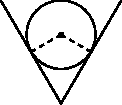
\includegraphics[scale=1]{gesamttex/edit_VIII-4/images/LBr_724_018-019_d4_018v.pdf}
\hfill
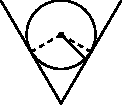
\includegraphics[scale=1]{gesamttex/edit_VIII-4/images/LBr_724_018-019_d5_018v.pdf}
\hfill
\edcaption{\lbrack\textit{Fig.~4}\rbrack 
\hspace{40mm}%
\lbrack\textit{Fig.~5}\rbrack}
\end{edfigure}
\pstart
Replicari\edlabel{LBr_724_018-019_3b}
posse
\edtext{videtur ad \textls{primum} equidem cessare instantiam aut saltem esse immutandam, si 
\indexN{\textls{Vanni}, Giovanni Francesco 1638\textendash1709}autor 
\cite{01995}\textit{Speciminis} additionem}{%
\lemma{videtur}%
\Bfootnote{%
\bars{ad \textls{primum} \textit{erg.}} equidem
\textit{(1)}~cessare %
\textit{(2)}~omitti posse %
\textit{(3)}~cessare instantiam %
\bars{aut \bars{aut \textit{gestr.}} saltem esse immutandam \textit{erg.}} , si autor \textit{Speciminis}
\textit{(a)}~assertionem suam
\textit{(b)}~additionem~\textit{L}}}
momentorum\indexS{additio momentorum}
\edtext{quibus grave\indexS{grave} in plano declivi descendere conatur,\indexS{grave in plano declivi descendens} et in alterum planum agit,\indexS{grave in planum declive agens}}{%
\lemma{}%
\Bfootnote{%
quibus grave in plano declivi descendere conatur, et in alterum planum agit, %
\bars{et recte quidem, \textit{gestr.}} %
\textit{erg.~L}}}
ad solum angulum rectum planorum\indexS{angulus planorum rectus}
\edtext{restringat, itaque si vires\indexS{vis} solum considerandae hic essent\lbrack,\rbrack\ additio}{%
\lemma{restringat,}%
\Bfootnote{%
\bars{in quo recte fecit \textit{erg.~u.~gestr.}} %
\textit{(1)}~qu %
\textit{(2)}~non tamen sine ratione objectum fuisse, %
\textit{(a)}~quia revera etiam in aliis planis %
\bars{alium angulum facientibus, \textit{erg.}} ex %
\textit{(aa)}~prem %
\textit{(bb)}~momentis quibus singula plana premuntur %
additio momentorum locum habet,
\textit{(b)}~si rigidius agere %
\textit{(c)}~et in rigore %
\textit{(aa)}~augeri posse %
\textit{(bb)}~angulum augeri posse %
\textit{(3)}~secu %
\textit{(4)}~additio momentorum \bars{locum \textit{streicht Hrsg.}} %
\textit{(5)}~itaque si %
\bars{secundum mentem \textit{Speciminis} \textit{erg.~u.~gestr.}} %
vires solum considerandae hic essent additio~\textit{L}}}
\edtext{partialium}{%
\lemma{}%
\Bfootnote{%
partialium %
\textit{erg.~L}}}
momentorum\indexS{additio momentorum partialium} locum
\edlabel{LBr_724_018-019_7a}%
\edtext{}{%
\xxref{LBr_724_018-019_7a}{LBr_724_018-019_7b}%
\lemma{habet,}%
\Bfootnote{%
\textit{(1)}~licet singula aliter sint aestimanda quam autor fecit. Non vero negatum est %
\textit{(2)}~quibus premuntur plana, sed ex merito distinguuntur ab his quibus %
\textit{(3)}~et, si %
\textit{(a)}~vis %
\textit{(aa)}~qua plana premuntur ea est secund %
\textit{(bb)}~quam grave exercet %
\textit{(cc)}~qua %
\textit{(aaa)}~grave in plano declivi descen %
\textit{(bbb)}~grave in plano %
agit ea est qua %
premit, ea est, qua %
\textit{(b)}~vires quibus grave in plano premit, eae essent, quibus %
\textit{(4)}~quibus grave %
\textit{(a)}~planum %
\textit{(b)}~in declivibus planis descendere conatur. %
\textit{(aa)}~Utique secundum %
\textit{(aaa)}~men %
\textit{(bbb)}~rationes autoris %
\textit{(bb)}~Quemadmodum pon %
\textit{(cc)}~Utique semper %
\textit{(aaa)}~ea in unam summam addenda esset, %
\textit{(bbb)}~eae in unam summam addendae essent,  %
quicumque sit angulus, alioqui aliquod earum %
\textit{(aaaa)}~periret %
\textit{(bbbb)}~perirent  %
\textit{(cccc)}~periret %
nihil agendo. Sed recte notavit \href{\Scan{LBr_724_19r}}%
{\lbrack19~r\textsuperscript{o}\rbrack} %
\textit{(aaaaa)}~et %
\textit{(bbbbb)}~Adm.\,R.\,P.~Kochanskius etiam illas vires in computum venire debere quibus grave %
\textit{(aaaaa-a)}~pla %
\textit{(bbbbb-b)}~in plano %
\textit{(aaaaa-aa)}~des %
\textit{(bbbbb-bb)}~declivi descendens ipsum planum declive premit, nec addenda esse simpliciter momenta, %
\textit{(aaaaa-aaa)}~alioqui fieret summa major %
\textit{(bbbbb-bbb)}~quae in rationes veniunt, %
\textit{(aaaaa-aaaa)}~et quae locum haberent; si unum tantum planum adesset %
\textit{(bbbbb-bbbb)}~sed quantitates tantum ipsis proportionales. %
\href{\Scan{LBr_724_18v}}%
{\lbrack18~v\textsuperscript{o}\rbrack} %
\textit{(dd)}~Ad \textls{secundum} replicatur: negatum non esse~\textit{L}}}%
habet, quibus grave in declivibus planis\indexS{planum declive} descendere conatur.\indexS{grave in plano declivi descendens}
\pend
\pstart
Ad \textls{secundum} replicatur: negatum non esse%
\edlabel{LBr_724_018-019_7b}
\edtext{momenta\indexS{momentum} quaecunque in unum posse addi,\indexS{additio momentorum} %
\edtext{sed ab \indexN{\textls{Vanni}, Giovanni Francesco 1638\textendash1709}autore \lbrack in\rbrack\ unum}{%
\lemma{sed}%
\Bfootnote{%
\textit{(1)}~ista %
\textit{(2)}~ab autore %
\bars{in \textit{gestr., wieder gültig gemacht Hrsg.}} %
unum~\textit{L}}}
addita aequari momento totali.\indexS{momentum totale} Negatum quoque non est}{%
\lemma{}%
\Bfootnote{%
momenta quaecunque \lbrack...\rbrack\ non est %
\textit{erg.~L}}}
momenta\indexS{momentum quo planum singulum premitur} quibus singula plana
\edtext{revera}{%
\lemma{}%
\Bfootnote{%
revera %
\textit{erg.~L}}}
premuntur,
\edtext{in unum addita\indexS{additio momentorum}}{%
\lemma{in unum}%
\Bfootnote{%
\textit{(1)}~adda %
\textit{(2)}~addita~\textit{L}}}
componere
\edtext{totale\indexS{momentum totale seu absolutum} seu absolutum momentum globi, nam id quoque per se patet cum tota vis\indexS{vis globi} globi a planis sustineatur,}{%
\lemma{totale}%
\Bfootnote{%
\textit{(1)}~momentum, %
\textit{(2)}~seu absolutum momentum globi, %
\textit{(a)}~sed hoc tantum, quod %
\textit{(b)}~id enim per se patet, %
\textit{(c)}~nam id \lbrack...\rbrack\  sustineatur,~\textit{L}}}
sed hoc tantum 
\edtext{negatur\lbrack:\rbrack}{%
\lemma{}%
\Bfootnote{%
negatur\lbrack:\rbrack\ %
\textit{erg.~L}}}
ea momenta
\edtext{quibus grave\indexS{grave} planum alterutrum\lbrack,\rbrack\ si cedere posset, propelleret,\indexS{momentum quo grave in planum agit}}{%
\lemma{quibus}%
\Bfootnote{%
\textit{(1)}~in singulis %
\textit{(2)}~singula plana propelleret %
\textit{(a)}~si posset %
\textit{(b)}~grave si posset %
\textit{(aa)}~grave \bars{alterutrum \textit{gestr.}} %
\textit{(bb)}~planum alterutrum\lbrack,\rbrack\ si cedere posset, propelleret,~\textit{L}}}
hoc est, (in casu recti
\edtext{planorum}{%
\lemma{}%
\Bfootnote{%
planorum %
\textit{erg.~L}}}
anguli),\indexS{angulus planorum rectus} 
\edtext{momenta}{%
\lemma{}%
\Bfootnote{%
momenta %
\textit{erg.~L}}}
\edtext{quibus in altero plano declivi descenderet,\indexS{grave in plano declivi descendens} si posset\lbrack,\rbrack}{%
\lemma{quibus in}%
\Bfootnote{%
\textit{(1)}~opposito %
\textit{(2)}~altero plano declivi %
\textit{(a)}~descendit, si possit %
\textit{(b)}~descenderet, si posset~\textit{L}}}
coincidere cum his quibus ipsa plana in casu impediti descensus\indexS{descensus impeditus}
\edtext{premuntur, ac proinde}{%
\lemma{premuntur,}%
\Bfootnote{%
\textit{(1)}~seu %
\textit{(2)}~ac proinde~\textit{L}}}
in unum addita\indexS{additio momentorum}
\edtext{\lbrack momentum\rbrack}{%
\lemma{}%
\Bfootnote{%
planum %
\textit{L ändert Hrsg.}}}
totale\indexS{momentum totale}
\edtext{conficere.\edlabel{LBr_724_018-019_13b} %
\href{\Scan{LBr_724_19r}}%
{\lbrack19~r\textsuperscript{o}\rbrack} Et recte}{%
\lemma{conficere.}%
\Bfootnote{%
\textit{(1)}~Verum %
\textit{(2)}~Nec puta %
\textit{(3)}~Placet \bars{autem \textit{gestr.}} %
ex multis modis quibus demonstrari %
\textit{(a)}~solet potestque %
\textit{(b)}~potest communis regula Staticorum quam autor \textit{Speciminis} impugnat, unam %
\bars{non inelegantem \textit{erg.}} 
\bars{,~nec quantum meminerim \textit{erg.~u.~gestr.}} %
hoc loco adducere ut si satisfacere ei autor non potest, %
\textit{(aa)}~agnoscat assumtam 
\textit{(aaa)}~illam
\textit{(bbb)}~ab ipso momentorum additionem, quae sola in demonstratione ejus, jam super negari potest, jure negatam fuisse. 
\textit{(bb)}~agnoscat non temere sibi contradici.
\textit{(4)}~Ut autem
\textit{(a)}~hoc jure negari %
\textit{(aa)}~(quod enim demonstravi) %
\textit{(bb)}~(cui enim demonst %
\textit{(cc)}~(in quo %
\textit{(dd)}~( quod 
\textit{(aaa)}~\textlangle\textendash\textrangle\ %
\textit{(bbb)}~potissimam in demonstratione \textit{Speciminis} dubitationem accipit, %
\textit{(b)}~additionem ab autore docto \textit{Speciminis}  %
\textit{(aa)}~propositam %
\textit{(bb)}~sine probationem propositam %
\bars{jure negari appareat \textit{streicht Hrsg.}}
\href{\Scan{LBr_724_19r}}%
{\lbrack19~r\textsuperscript{o}\rbrack} Et recte~\textit{L}}}
\edtext{notavit \indexN{\textls{Kochański}, Adam Adamandus 1631\textendash1700}Adm.\,R.\,P.~Kochanskius in \cite{01023}\textit{Actis} Jun. 1685.}{%
\lemma{notavit \lbrack...\rbrack\ 1685}%
\Cfootnote{\indexN{\textls{Kochański}, Adam Adamandus 1631\textendash1700}\textsc{A.\,A. Kochański}, %
\cite{01996}\textit{Consideratio speciminis libri de momentis gravium, Authore J.\,F.\,V. Lucensi}, %
\cite{01023}\textit{Acta eruditorum},
Juni 1685, S.\;262\textendash265.}}
etiam illa momenta consideranda esse, quibus grave
\edtext{etiam}{%
\lemma{}%
\Bfootnote{etiam \textit{erg.~L}}}
in plano declivi decurrens\indexS{grave in plano declivi decurrens} hoc planum
\edtext{premit,\indexS{momentum quo grave planum premit} praeterea non}{%
\lemma{premit,}%
\Bfootnote{%
\textit{(1)}~nec %
\textit{(2)}~praeterea non~\textit{L}}}
simpliciter addenda esse
\edtext{momenta\indexS{additio momentorum} illa}{%
\lemma{momenta}%
\Bfootnote{%
\textit{(1)}~qualia ess %
\textit{(2)}~illa~\textit{L}}}
quae in rationes
\edtext{veniunt alioqui summa excederet momentum totale,\indexS{momentum totale} sed quantitates proportionales}{%
\lemma{veniunt}%
\Bfootnote{%
\textit{(1)}~sed quantitates e %
\textit{(2)}~alioqui summa excederet momentum totale, sed quantitates %
\textit{(a)}~proportionis %
\textit{(b)}~proportionales~\textit{L}}}
in quas momentum totale\indexS{momentum totale}
\edtext{distribuitur. \href{\Scan{LBr_724_18v}}%
{\lbrack18~v\textsuperscript{o}\rbrack} Quoniam}{%
\lemma{distribuitur.}%
\Bfootnote{%
\textit{(1)}~Ut autem eam additionem quae potissimam in demonstratione %
\textit{Speciminis} dubitationem recipit jure negari appareat %
\textit{(2)}~\href{\Scan{LBr_724_18v}}%
{\lbrack18~v\textsuperscript{o}\rbrack} Quoniam~\textit{L}}}
autem testatur doctissimus \indexN{\textls{Vanni}, Giovanni Francesco 1638\textendash1709}autor
\edtext{\cite{01995}\textit{Speciminis} demonstrationes regulae}{%
\lemma{\textit{Speciminis}}%
\Bfootnote{%
\textit{(1)}~quasdam %
\textit{(2)}~demonstrationes %
\textit{(a)}~quas refert %
\textit{(b)}~regulae~\textit{L}}}
staticorum\indexS{regula staticorum}
\edtext{quas apud \indexN{\textls{Galilei} (Galilaeus, Galileus), Galileo 1564\textendash1642}Galilaeum 
et \indexN{\textls{Torricelli} (Torricellius), Evangelista 1608\textendash1647}Torricellium extare ait,}{%
\lemma{quas \lbrack...\rbrack\ ait}%
\Cfootnote{\textsc{Vanni},\indexN{\textls{Vanni}, Giovanni Francesco 1638\textendash1709} \cite{01995}\textit{Specimen} hier S.\;511.
Siehe
\indexN{\textls{Galilei} (Galilaeus, Galileus), Galileo 1564\textendash1642}%
\textsc{G.~Galilei}, %
\cite{00050}\textit{Discorsi}, %
Giornata Terza, De motu naturaliter accelerato; \glqq Aggiunta postuma dell'Autore\grqq\ %
nach dem Scholion zum 2.~Theorem (der Zusatz erschien erst in der posthumen Werkausgabe: \cite{01084}\textit{Opere}, Bologna 1656, Bd.~II, S.\;132\lbrack ter\rbrack\textendash134; \cite{00048}\textit{GO} VIII, S.\;216\textendash219 im Apparat) %
und 
\indexN{\textls{Torricelli} (Torricellius), Evangelista 1608\textendash1647}%
\textsc{E.~Torricelli}, \textit{De motu gravium}, lib.~I
(\cite{00304}\textit{Opera geometrica}, Florenz 1644, S.\;99;
\cite{00108}\textit{TO}~II, S.\;105).}}
sibi parum solidas visas, eaeque mihi non sunt ad manus\lbrack,\rbrack\ 
placet aliquam subjicere, quae videtur manifesta, nec inelegans.
\pend
\begin{edfigure}%
\hfill
\includegraphics[scale=1]{%
gesamttex/edit_VIII-4/images/LBr_724_018-019_d6_018v.pdf}
\hfill
\includegraphics[scale=1]{%
gesamttex/edit_VIII-4/images/LBr_724_018-019_d7_018v.pdf}
\hfill
\edcaption{\lbrack\textit{Fig.~6}\rbrack 
\hspace*{40mm}%
\edtext{\lbrack\textit{Fig.~7, gestr.}\rbrack}{%
\lemma{\lbrack\textit{Fig.~7}\rbrack}%
\Cfootnote[nonum]{%
Ein ebenfalls gestrichener Entwurf zum Diagramm wird nicht wiedergegeben.}}}
\end{edfigure}
\pstart
\noindent
\lbrack%
\textit{Nachfolgend kleingedruckter Text (erste Fassung des Beweises %
auf \refpassage{LBr_724_018-019_10a}{LBr_724_018-019_10b}) samt Zeichnungen gestrichen:}\rbrack
\pend
\vspace{0.5em}
\footnotesize
\pstart 
\noindent
Suppono autem, corporibus duobus ita positis, ut 
uno ascendente alterum descendat,\indexS{corpus ascendens altero corpore descendente} et contra, nullum 
fieri motum a gravitate,\indexS{gravitas} nisi plus descendat quam ascendat, 
seu nisi descendat commune eorum centrum gravitatis.\indexS{centrum gravitatis commune}
Assumo etiam Lemma
\edlabel{LBr_724_018-019_4a}%
\edtext{}{%
\xxref{LBr_724_018-019_4a}{LBr_724_018-019_4b}%
\lemma{Geometricum}%
\Bfootnote{%
\textit{(1)}~facile demonstratu %
\textit{(2)}~ni fallor elegans. %
\textit{(a)}~\bars{Si \textit{streicht Hrsg.}} in basi trianguli sumatur punctum %
\textit{(b)}~Si duorum trianguli laterum uni %
\textit{(aa)}~tantum adda %
\textit{(bb)}~producto tantum addatur quantum ab \bars{altero \textit{streicht Hrsg.}} abscinditur %
\textit{(c)}~Duorum triangulorum %
\textit{(d)}~Si triangula quaecunque %
\textit{(e)}~Omnium triangulorum angulum congruentem et summam%
\textit{(aa)}~laterum %
\textit{(bb)}~crurum %
eandem habentium bases %
\textit{(aaa)}~ab eadem recta, %
\textit{(aaaa)}~eaque ad alterutrum %
\textit{(aaaaa)}~lat %
\textit{(bbbbb)}~crus (quod productum omni %
\textit{(bbbb)}~in eadem ratione secantur, eaque est perpendicularis ad %
\textit{(bbb)}~a recta ad crus %
\textit{(aaaa)}~commune perpendicu %
\textit{(bbbb)}~si producatur %
\textit{(cccc)}~commune perpendiculari in eadem ratione secantur. %
\textit{(aaaaa)}~Si trian %
\textit{(bbbbb)}~Sit triangulum \textit{ABC} sumaturque %
\textit{(aaaaa-a)}~ver %
\textit{(bbbbb-b)}~a \textit{C} versus \textit{A} %
\textit{(ccccc-c)}~in \textit{AC} a \textit{C} versus \textit{A} punctum \textit{D}, et in \textit{AB} produc %
\textit{(ccccc)}~Hoc est si sint triangula \textit{ABC} %
et \textit{ADE}, et \textit{EC} aequalis \textit{BD} %
cadant autem \textit{E} in rectam \textit{AC}, et \textit{B} in rectam \textit{AD} et ex %
\bars{uno \textit{gestr.}} crure communi ut \textit{AB}, educatur perpendicularis %
aliqua \textit{FGH} secans \textit{DE} in \textit{G}, et \textit{BC} in \textit{H}, erit %
$DG : GE\; \squaredots\; BH : HC$.
\href{\Scan{LBr_724_19r}}%
{\lbrack19~r\textsuperscript{o}\rbrack}
\textit{(f)}~Duorum triangulorum~\textit{L}}}%
Geometricum ni fallor elegans.
\pend
\normalsize
\begin{edfigure}%
\includegraphics[scale=1]{%
gesamttex/edit_VIII-4/images/LBr_724_018-019_d8_018v.pdf}
\edcaption{\edtext{\lbrack\textit{Fig.~8, gestr.}\rbrack}{%
\lemma{\lbrack\textit{Fig.~8}\rbrack}%
\Cfootnote[nonum]{Das Diagramm wird von Leibniz lediglich in gestrichenen Varianten besprochen: Siehe die Variante \textit{(e)}, bes. \textit{(ccccc)} zu \refpassage{LBr_724_018-019_4a}{LBr_724_018-019_4b}.}}}
\end{edfigure}
\pstart 
\noindent
\href{\Scan{LBr_724_19r}}%
{\lbrack19~r\textsuperscript{o}\rbrack}
\pend
\begin{edfigure}[0.25em][1em]    	%
\hfill
\includegraphics[scale=1]{%
gesamttex/edit_VIII-4/images/LBr_724_018-019_d9_019r.pdf}
\hfill
\includegraphics[scale=1]{%
gesamttex/edit_VIII-4/images/LBr_724_018-019_d10_019r.pdf}
\hfill
\edcaption{%
\edtext{\lbrack\textit{Fig.~9, gestr.}\rbrack}{%
\lemma{\lbrack\textit{Fig.~9}\rbrack}%
\Cfootnote[nonum]{Ein ebenfalls gestrichener Entwurf zum Diagramm wird nicht wiedergegeben.}}
\hspace*{28mm}%
\edtext{\lbrack\textit{Fig.~10, gestr.}\rbrack}{%
\lemma{\lbrack\textit{Fig.~10}\rbrack}%
\Cfootnote[nonum]{Ein ebenfalls gestrichener Entwurf zum Diagramm wird nicht wiedergegeben.}}}
\end{edfigure}
\footnotesize
\pstart
Duorum triangulorum
\edlabel{LBr_724_018-019_4b}
\edtext{angulum coincidentem et summa crurum}{%
\lemma{angulum}%
\Bfootnote{%
\textit{(1)}~congruentem %
\textit{(2)}~coincidentem et summa %
\textit{(a)}~crurum eandem habentium %
\textit{(b)}~laterum eandem habentium %
\textit{(c)}~crurum~\textit{L}}}
circa eum angulum communem habentium latera se
\edtext{mutuo}{%
\lemma{}%
\Bfootnote{%
mutuo %
\textit{erg.~L}}}
secant in eadem
\edtext{ratione. Seu si duarum}{%
\lemma{ratione.}%
\Bfootnote{%
\textit{(1)}~Si sint duae rectae in eodem plano positae inter se aequales per quatuor eorum puncta extrema circulus describi potest
\textit{(2)}~Seu si~\textit{L}}}
rectarum aequalium in eodem plano
\edtext{positarum}{%
\lemma{}%
\Bfootnote{%
positarum %
\textit{erg.~L}}}
extrema jungantur rectae jungentes sese secabunt in eadem 
\edtext{ratione. $AB : CD\; \squaredots\; BE : CD$. Ergo}{%
\lemma{ratione.}%
\Bfootnote{%
\textit{(1)}~Hinc %
\textit{(2)}~Eritq %
\textit{(3)}~$AB : CD\; \squaredots\; BE : $
\textit{(a)}~\textit{GF}. Ergo $AB : BE\; \squaredots\; CD : GF\; \squaredots\; LC$ 
\bars{:~\textit{LG} \textit{gestr.}} %
\textit{(b)}~\textit{CD}. Ergo~\textit{L}}}
\textit{AB} aeq.~\textit{BE}.
\pend
\normalsize
\vspace{0.5em} %
\pstart
\noindent
\lbrack%
\textit{Nachfolgend kleingedruckter Text (zweite Fassung des Beweises %
auf \refpassage{LBr_724_018-019_10a}{LBr_724_018-019_10b}) gestrichen:}\rbrack
\pend
\vspace{0.5em}
\footnotesize
\pstart 
\noindent
Suppono
\edtext{autem duobus}{%
\lemma{autem}%
\Bfootnote{%
\textit{(1)}~corporibus %
\textit{(2)}~duobus~\textit{L}}}
gravibus ita positis, ut uno ascendente alterum
descendere necesse sit,\indexS{corpus ascendens altero corpore descendente} nullum fieri motum
a gravitate,\indexS{gravitas} nisi potior sit ascensus quam descensus,
seu nisi descendat eorum centrum gravitatis\indexS{centrum gravitatis commune}
\edlabel{LBr_724_018-019_5a}%
\edtext{}{%
\xxref{LBr_724_018-019_5a}{LBr_724_018-019_5b}%
\lemma{commune.}%
\Bfootnote{%
\textit{(1)}~Sit recta verticalis %
\textit{(1)}~\textit{AB} %
\textit{(2)}~\textit{ADBF}, et recta declivis \textit{AGCE}, %
\textit{(a)}~et gravia \textit{B} et \textit{C}, connexa fune \textit{BAC} %
\textit{(b)}~et gravia %
\textit{F} et \textit{G} sint in aequilibrio, junctaque \textit{FG}, sit
\textit{(aa)}~centrum %
\textit{(bb)}~gravium %
\textit{F} et \textit{G} centrum gravitatis. Jam si gravia %
\textit{F} et \textit{G} sunt in aequilibrio, manebunt in aequilibrio %
\textit{(aaa)}~etiamsi fune prehenso \textit{G} detrahas in \textit{E},  %
\textit{(bbb)}~translato \textit{F} in \textit{D} et \textit{G} in \textit{E}, si scilicet prehenso fune %
\textit{(aaaa)}~det %
\textit{(bbbb)}~detrahas \textit{G} in \textit{E} %
\textit{(ccc)}~etiamsi prehenso \lbrack...\rbrack\ \textit{E}, %
\textit{(aaaa)}~eademque %
\textit{(bbbb)}~simulque attollas \textit{F} in \textit{D} %
\textit{(aaaaa)}~, existente %
\textit{(bbbbb)}~. Ergo centrum gravitatis %
\textit{(aaaaa-a)}~ipsorum \textit{D} et \textit{H} in eadem est %
\textit{(bbbbb-b)}~manet in eadem semper altitudine, quae erat ipsius \textit{H}, %
seu ducta per \textit{H} recta horizontali \textit{BHC}, quae verticali ad angulos %
rectos occurrat in \textit{B}, declivi occurrat in \textit{C}, centrum gravitatis %
ipsorum \textit{D} et \textit{E}, erit in eadem recta \textit{BC}, in qua centrum \textit{H}. %
Et si grave \textit{F} vel \textit{D} %
\textit{(2)}~Sit recta~\textit{L}}}%
commune.
\pend
\normalsize
\begin{edfigure}[1em][1em]    	%
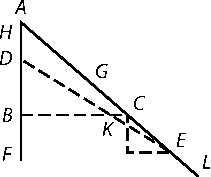
\includegraphics[scale=1]{gesamttex/edit_VIII-4/images/LBr_724_018-019_d11_019r.pdf}
\edcaption{\edtext{\lbrack\textit{Fig.~11, nicht gestr.}\rbrack}{\lemma{}%
\Afootnote{\textit{Am Rand, neben \lbrack\textit{Fig.~11}\rbrack, ebenfalls nicht gestrichen:} si sit \textit{CE} aeq.\ \textit{BD} et \textit{DE} secet \textit{BC} in \textit{K}, erit $EK : KD\; \squaredots\; BA : AC$.}}}
\end{edfigure}
\footnotesize
\pstart
Sit recta\edlabel{LBr_724_018-019_5b}
verticalis \textit{ADBF}, et declivis
\edtext{\textit{AGCE}, et angulus}{%
\lemma{\textit{AGCE},}%
\Bfootnote{%
\textit{(1)}~sintque dua gravia \textit{B} et %
\textit{(2)}~et angulus~\textit{L}}}
\edtext{%
\textit{ABC} rectus, sintque duo
gravia\indexS{gravia fune connexa} \textit{B} et \textit{C}, fune\indexS{funis}
\edtext{\textit{BAC} connexa eaque in aequilibrio.\indexS{gravia in aequilibrio} Erit}{%
\lemma{\textit{BAC}}%
\Bfootnote{%
\textit{(1)}~, verticali %
\textit{(2)}~connexa eaque in aequilibrio. %
\textit{(a)}~Erit utique %
\textit{(b)}~Erit~\textit{L}}}
eorum centrum gravitatis\indexS{centrum gravitatis gravium} in recta
\edtext{jungente, \textit{BC}.}{%
\lemma{jungente,}%
\Bfootnote{%
\textit{(1)}~\textit{BH} %
\textit{(2)}~\textit{BC}.~\textit{L}}}
Manent autem in aequilibrio,\indexS{aequilibrium} etiamsi fune\indexS{funis} apprehenso detrahas
\textit{C} in \textit{E}, simulque attollas \textit{B} in \textit{D},
\edtext{existentibus}{%
\lemma{existentibus}%
\Bfootnote{%
\textit{(1)}~\textit{CD} %
\textit{(2)}~\textit{CE},~\textit{L}}}
\textit{BD} aequalibus; (vel etiamsi detrahas \textit{B} in \textit{F} simulque attollas \textit{C} in \textit{G}
existentibus \textit{BF},
\edtext{\textit{CG} aequalibus)}{%
\lemma{\textit{CG}}%
\Bfootnote{%
\textit{(1)}~) %
\textit{(2)}~aequalibus)~\textit{L}}}
itaque etiam centrum}{\lemma{}\Afootnote{%
\textit{Am Rand, nicht gestrichen:} NB multa elegantia Lemmata Geometrica ex his duci possent ut quod recta \textit{BC} ipsas \textit{DE}, \textit{FG}, \textit{HL} in eadem ratione secat\textsuperscript{\lbrack a\rbrack} quae est \textit{AC} ad \textit{AB}, si \textit{BD} et \textit{CE}, item \textit{BF} et \textit{CG} item \textit{BH} et \textit{CL}, sint aequales.
\\[1.5ex]%
{\footnotesize \textsuperscript{\lbrack a\rbrack} secat \bars{quae est \textit{AC} ad \textit{AB} \textit{erg.}}, %
\textit{(1)}~si \textit{BF} et \textit{CG}, %
\textit{(2)}~si \textit{BD} \textit{L}}}}
gravitatis\indexS{centrum gravitatis commune} semper manebit in eadem altitudine, nempe in
\edtext{recta BC,}{%
\lemma{recta}%
\Bfootnote{%
\textit{(1)}~\textit{BH} %
\textit{(2)}~\textit{BC},~\textit{L}}}
sive situs gravium sit \textit{B}, \textit{C}; sive
\edtext{\textit{D}, \textit{E}; sive}{%
\lemma{\textit{D}, \textit{E};}%
\Bfootnote{%
\textit{(1)}~si \textit{F}, \textit{G} %
\textit{(2)}~sive~\textit{L}}}
\textit{F}, \textit{G}.
\pend
\pstart
Quod si ergo grave \textit{B} 
\edtext{attollas in \textit{H},}{%
\lemma{attollas}%
\Bfootnote{%
\textit{(1)}~per %
\textit{(2)}~in %
\textit{(a)}~\textit{A} %
\textit{(b)}~\textit{H}~\textit{L}}}
ita ut quantillum vis\indexS{vis} absit ab \textit{A}, detrahasque simul \textit{C} in \textit{L}, ita ut
\edtext{\textit{CL} sit aequal.~\textit{BH}\lbrack,\rbrack}{%
\lemma{\textit{CL} sit}%
\Bfootnote{%
\textit{(1)}~aeq.~\textit{B} %
\textit{(2)}~aequal.~\textit{BH}~\textit{L}}}
patet, centrum
\edtext{gravitatis\indexS{centrum gravitatis commune} gravium \textit{H} et \textit{L} cadere adhuc}{%
\lemma{gravitatis}%
\Bfootnote{%
\textit{(1)}~ipsorum %
\textit{(2)}~gravium \textit{H} et \textit{L} cadere %
\textit{(a)}~in rectam \textit{BC} %
\textit{(b)}~adhuc~\textit{L}}}
in
\edtext{rectam \textit{BC}, idem}{%
\lemma{rectam \textit{BC},}%
\Bfootnote{%
\textit{(1)}~idemque cadere in rectam \textit{HL} %
\textit{(2)}~idem~\textit{L}}}
autem cadit in rectam \textit{HL} 
\edtext{et proinde in rectarum \textit{BC}, \textit{HL} intersectionem,}{%
\lemma{}%
\Bfootnote{%
et proinde in rectarum \textit{BC}, \textit{HL} intersectionem, %
\textit{erg.~L}}}
ergo
\edtext{quo \textit{H} propius}{%
\lemma{quo}%
\Bfootnote{%
\textit{(1)}~propius \textit{H} a %
\textit{(2)}~\textit{H} propius~\textit{L}}}
assumseris ad \textit{A}, erit centrum gravitatis\indexS{centrum gravitatis commune} ipsorum \textit{H}, \textit{L}, propius
\edtext{ipsi \textit{C}, efficereque}{%
\lemma{ipsi \textit{C},}%
\Bfootnote{%
\textit{(1)}~ita ut tantum absit a %
\textit{(2)}~efficereque~\textit{L}}}
possumus ut absit
\edtext{a \textit{C} intervallo}{%
\lemma{a \textit{C}}%
\Bfootnote{%
\textit{(1)}~errore qui sit %
\textit{(2)}~intervallo~\textit{L}}}
quod sit minus quovis dato,
et denique si \textit{H} incidat in \textit{A}, erit \textit{CL}, aeq.~\textit{BA}, centrumque %
gravitatis\indexS{centrum gravitatis commune} ipsorum \textit{H} et \textit{L} incidet in \textit{C},
\edtext{intersectionem rectarum \textit{BC}, et \textit{HL}\lbrack,\rbrack}{%
\lemma{}%
\Bfootnote{%
intersectionem rectarum \textit{BC}, et \textit{HL} %
\textit{erg.~L}}}
ergo grave \textit{L} sive \textit{C} erit
\edtext{ad grave \textit{H}}{%
\lemma{ad grave}%
\Bfootnote{%
\textit{(1)}~\textit{B} sive %
\textit{(2)}~\textit{H}~\textit{L}}}
seu \textit{A} sive \textit{B}, ut \textit{AC} ad \textit{CL} sive \textit{BC}.
Quod erat demonstrandum.
\pend
\pstart
Demonstrationem autem brevitatis
\edtext{ac claritatis}{%
\lemma{ac}%
\Bfootnote{%
\textit{(1)}~claritatisque %
\textit{(2)}~claritatis~\textit{L}}}
causa exposui familiarius; si quis vero pertinacius
\edtext{resistat, facile}{%
\lemma{resistat,}%
\Bfootnote{%
\textit{(1)}~ex his %
\textit{(2)}~faci %
\textit{(3)}~facile~\textit{L}}}
ad absurdum redigi potest, eo ipso
\edtext{quod discrimen}{%
\lemma{quod}%
\Bfootnote{%
\textit{(1)}~discrimen ab eo quod asserimus dato quovis minus \bars{esse \textit{streicht Hrsg.}} ostendi potest %
\textit{(2)}~discrimen
~\textit{L}}}
a sententia nostra dato quovis minus esse ostendi potest.
\pend
\normalsize %
\vspace{0.5em} %
\newpage
\pstart
\centering 
\edlabel{LBr_724_018-019_9a}%
\edtext{}{%
\xxref{LBr_724_018-019_9a}{LBr_724_018-019_9b}%
\lemma{\href{\Scan{LBr_724_19v}}%
{\lbrack19~v\textsuperscript{o}\rbrack}}%
\Bfootnote{%
\textit{(1)}~Cum vir quidam %
\textit{(a)}~doc %
\textit{(b)}~doctus %
\textit{(c)}~ingeniosissi %
\textit{(d)}~doctus %
eam regulam nuper in dubium revocaverit \textit{Specimine} edito %
\textit{(aa)}~in %
\textit{(aaa)}~mom %
\textit{(bbb)}~sche %
\textit{(bb)}~\textit{de momentis gravium} %
inserto in \textit{Actis} Novembr.~1684.\ placet ex compluribus  %
\bars{regulae \textit{erg.}} %
demonstrationibus unam %
\bars{prae alteras \textit{gestr.}} %
non inelegantem subjicere, ut appareat quid ad eam %
\textit{(aaa)}~vir doctus %
\textit{(bbb)}~autor \textit{Speciminis} %
excipere possit. %
\textit{(2)}~Demonstratio %
\textit{(a)}~communis %
\textit{(b)}~Geometrica~\textit{L}}}%
\href{\Scan{LBr_724_19v}}%
{\lbrack19~v\textsuperscript{o}\rbrack} %
\hfill
\edlabel{LBr_724_018-019_10a}%
Demonstratio Geometrica%
\edlabel{LBr_724_018-019_9b}
regulae apud staticos\indexS{statici} receptae\indexS{regula apud staticos recepta}
\hfill
\phantom{\lbrack19~v\textsuperscript{o}\rbrack}
\linebreak
de momentis gravium\indexS{momenta gravium in planis inclinatis} in planis inclinatis
\pend
\pstart
\noindent
\edtext{Sit planum verticale\indexS{planum verticale} \textit{ADB}, et inclinatum\indexS{planum inclinatum} \textit{ACE} et in illo descendere tendat grave\indexS{grave in plano declivi descendens} \textit{B}, in hoc}{%
\lemma{Sit }%
\Bfootnote{%
\textit{(1)}~recta verticalis \textit{ADBF}, et inclinata \textit{AGCE} et in illa
\textit{(a)}~grave \textit{B}, in hac grave \textit{D}, descendere tendens %
\textit{(b)}~descendere tendat grave \textit{B}, in hac %
\textit{(2)}~planum verticale \lbrack...\rbrack\ in hoc~\textit{L}}}
grave \textit{C},
\edtext{sint autem gravia}{%
\lemma{}%
\Bfootnote{%
sint autem gravia %
\textit{erg.~L}}}
connexa\indexS{gravia fune connexa} fune\indexS{funis}
\edtext{\textit{BAC}, angulusque \textit{ABC}}{%
\lemma{\textit{BAC},}%
\Bfootnote{%
\textit{(1)}~ponamusque eam esse rationem gravium inter se, ut %
\textit{(2)}~angulus autem %
\textit{(3)}~angulusque \textit{ABC}~\textit{L}}}
sit rectus, et gravia eam inter se rationem habeant ut sint in aequilibrio.\indexS{gravia in aequilibrio} 
Ajo fore grave \textit{B} ad grave \textit{C}, ut recta \textit{AB} ad 
\edlabel{LBr_724_018-019_11a}%
\edtext{}{%
\xxref{LBr_724_018-019_11a}{LBr_724_018-019_11b}%
\lemma{rectam \textit{AC}.}%
\Bfootnote{%
\textit{(1)}~Trahatur grave \textit{C} in \textit{E}, \bars{ut \textit{erg.}} %
assurgat \textit{B} in \textit{D}, %
\textit{(a)}~eruntque %
\textit{(b)}~ex %
\textit{(c)}~erunt %
\textit{(d)}~patet %
\textit{(e)}~centrum gra %
\textit{(2)}~Prehendendo funem manu \bars{in \textit{C} \textit{erg.}} %
trahendoque ex situ \textit{BAC} \bars{in \textit{streicht Hrsg.}} %
situm \textit{DAE} (translatis gravibus %
\textit{(3)}~Funem~\textit{L}}}%
rectam \textit{AC}.
\pend
\begin{edfigure}[1em][1em]    	%
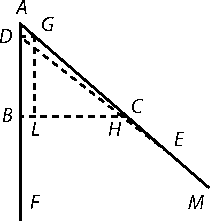
\includegraphics[scale=1]{gesamttex/edit_VIII-4/images/LBr_724_018-019_d12_019v.pdf}
\edcaption[0.25em]{\lbrack\textit{Fig.~12}\rbrack}
\end{edfigure}
\pstart
Funem\indexS{funis}%
\edlabel{LBr_724_018-019_11b}
(qui gravitate carere intellegitur) manu prehendendo
in \textit{C}, trahendoque grave \textit{C} deorsum
\edtext{in \textit{E}, adeoque simul}{%
\lemma{in \textit{E},}%
\Bfootnote{%
\textit{(1)}~simulque %
\textit{(2)}~adeoque simul~\textit{L}}}
grave \textit{B} sursum 
\edtext{in \textit{D}, (quo facto aequales erunt \textit{CE} et \textit{BD}) patet}{%
\lemma{in}%
\Bfootnote{%
\textit{(1)}~\textit{A}, %
\textit{(2)}~\textit{D}, %
\textit{(a)}~( %
\textit{(b)}~pat %
\textit{(c)}~sic ut %
\textit{(aa)}~sit aequa %
\textit{(bb)}~aequales sint \textit{CE} et \textit{BD}, patet %
\textit{(d)}~(quo facto \lbrack...\rbrack\ \textit{BD}) patet~\textit{L}}}
aequilibrium\indexS{aequilibrium} quod prius erat, inter gravia,
\edtext{manere; nec proinde eorum centrum gravitatis commune\indexS{centrum gravitatis commune} attolli vel deprimi.}{%
\lemma{manere;}%
\Bfootnote{%
\textit{(1)}~et similiter %
\textit{(2)}~nec \bars{proinde \textit{erg.}} eorum \lbrack...\rbrack\ deprimi.~\textit{L}}}
Cumque gravium in situ \textit{B}, \textit{C} centrum gravitatis\indexS{centrum gravitatis commune} esset in
\edtext{recta \textit{BC} horizontali, in ea manebit}{%
\lemma{recta \textit{BC}}%
\Bfootnote{%
\textit{(1)}~, utique non mutabitur %
\textit{(2)}~horizontali, %
\textit{(a)}~inque ea maneret %
\textit{(b)}~in ea manebit~\textit{L}}}
non obstante hac
\edtext{gravium translatione, quae ipsa in aequilibrio\indexS{gravia in aequilibrio} relinquit. Cumque sit}{%
\lemma{gravium}%
\Bfootnote{%
\textit{(1)}~translatione %
\textit{(a)}~, erit in intersectione %
\textit{(b)}~. Sitque %
\textit{(2)}~translatione, quae ipsa in aequilibrio relinquit. Cumque sit~\textit{L}}}
\edtext{praeterea idem centrum in recta}{%
\lemma{praeterea}%
\Bfootnote{%
\textit{(1)}~in recta %
\textit{(2)}~idem centrum in recta~\textit{L}}}
\textit{DE}, gravia in situ \textit{D}, \textit{E}, jungente,
\edtext{erit in rectarum \textit{BC}, \textit{DE}, intersectione \textit{H}. Jam}{%
\lemma{erit in}%
\Bfootnote{%
\textit{(1)}~earum intersectione \textit{H}. Constat autem ex %
\textit{(2)}~intersectione \textit{H} rectarum \textit{BC}, \textit{DE}, %
\textit{(3)}~rectarum \textit{BC}, \textit{DE}, intersectione \textit{H}. Jam~\textit{L}}}
ex Geometria\indexS{Geometria} ostendi
\edtext{potest lemma facile nec inelegans, si}{%
\lemma{potest}%
\Bfootnote{%
\textit{(1)}~esse %
\textit{(2)}~lemma %
\textit{(a)}~elegans, %
\textit{(b)}~faci %
\textit{(3)}~lemma facile nec inelegans,~\textit{L}}}
si sint \textit{CE}, \textit{BD} aequales, fore
$DH : HE\; \squaredots\;$%
\edtext{$AC : AB$. Est}{%
\lemma{$AC : AB$.}%
\Bfootnote{%
\textit{(1)}~Ergo et gravia %
\textit{(2)}~Sunt autem gravia \textit{E} et %
\textit{(3)}~Est~\textit{L}}}
autem ob aequilibrium gravium,\indexS{aequilibrium gravium}
\edtext{grave \textit{E} (sive \textit{C})}{%
\lemma{grave \textit{E}}%
\Bfootnote{%
\textit{(1)}~ad gra %
\textit{(2)}~(sive \textit{C})~\textit{L}}}
ad grave \textit{D} (sive \textit{B}) ut \textit{DH} ad \textit{HE},
quia \textit{H} est ipsorum \textit{D} et \textit{E} centrum gravitatis.\indexS{centrum gravitatis commune} Ergo
\edtext{erit grave \textit{C}}{%
\lemma{erit grave}%
\Bfootnote{%
\textit{(1)}~\textit{B} ad grave %
\textit{(2)}~\textit{C}~\textit{L}}}
ad grave \textit{B} ut \textit{AC} ad \textit{AB}.
\pend
\pstart
Idem
\edtext{aliter}{%
\lemma{}%
\Bfootnote{%
aliter %
\textit{erg.~L}}}
etiam sine assumto lemmate illo
\edtext{Geometrico ostendi potest, si grave \textit{B} attollatur usque ad \textit{A}, seu si}{%
\lemma{Geometrico}%
\Bfootnote{%
\textit{(1)}~ostendi potest, si %
\textit{(2)}~ostendi potest, si grave \textit{B} %
\textit{(a)}~erat %
\textit{(b)}~\bars{sive \textit{D} \textit{erg.}} eousque attollatur \textit{A} seu %
\textit{(c)}~attollatur usque ad \textit{A}, seu si~\textit{L}}}
(\textit{D}) incidat in ipsum punctum \textit{A},
\edtext{quo casu \textit{C}(\textit{E}) aequalis \textit{B}(\textit{D}) erit aequalis \textit{BA}, et (\textit{H})}{%
\lemma{quo}%
\Bfootnote{%
\textit{(1)}~casu (\textit{H}) %
\textit{(2)}~casu \textit{C}(\textit{E}) aequalis \textit{B}(\textit{D}) erit aequalis \textit{BA}, et (\textit{H})~\textit{L}}}
incidet in \textit{C}, et
\edtext{(\textit{H})(\textit{D}) coincidet cum \textit{CA}, eritque}{%
\lemma{(\textit{H})(\textit{D}) }%
\Bfootnote{%
\textit{(1)}~in \textit{CA} %
\textit{(2)}~coincidet cum \textit{CA}, %
\textit{(a)}~et 
\textit{(aa)}~\textit{CE} erit %
\textit{(aaa)}~aequ.~\textit{BD} %
\textit{(bbb)}~aequalis \textit{BA}
\textit{(bb)}~\textit{BD} erit aequalis \textit{BA}
\textit{(b)}~eritque~\textit{L}}}
gravium \textit{B} et \textit{C}
\edtext{nunc}{%
\lemma{}%
\Bfootnote{%
nunc %
\textit{erg.~L}}}
positorum in \textit{A} et (\textit{E}),
\edtext{centrum aequilibrii\indexS{centrum aequilibrii} \textit{C}}{%
\lemma{centrum}%
\Bfootnote{%
\textit{(1)}~gravitatis \textit{C}, %
\textit{(2)}~aequilibrii \textit{C}~\textit{L}}}
ac proinde (\textit{E}) sive \textit{C} ad \textit{B} sive \textit{A}, ut \textit{AC} ad \textit{C}(\textit{E}) sive \textit{AB}.
Placet tamen ipsius propositionis Geometricae demonstrationem
\edlabel{LBr_724_018-019_12a}%
\edtext{}{%
\xxref{LBr_724_018-019_12a}{LBr_724_018-019_12b}%
\lemma{subjicere. \lbrack/\rbrack}%
\Bfootnote{%
\textit{(1)}~Lemma \lbrack/\rbrack\ Si sint triangula %
\textit{(2)}~Lemma \lbrack/\rbrack\ Omnium triangulorum %
\bars{eundem \textit{gestr.}} angulum~\textit{L}}}%
subjicere.
\pend
\vspace{0.5\baselineskip}
\pstart%
\centering%
Lemma
\pend
\pstart
\noindent
Omnium triangulorum angulum\edlabel{LBr_724_018-019_12b}
coincidentem et summam laterum circa eundem angulum, aequalem habentium bases
a basi ejus trianguli quod inter ipsa rectangulum
\edtext{est in}{%
\lemma{}%
\Bfootnote{%
est \bars{est \textit{gestr.}} %
in~\textit{L}}}
eadem ratione secantur
\edtext{quae scilicet est ratio laterum}{%
\lemma{quae}%
\Bfootnote{%
\textit{(1)}~scilicet est ratio laterum %
\textit{(2)}~ratio scilicet est %
\textit{(3)}~eadem cum ratione %
\textit{(4)}~scilicet est ratio laterum~\textit{L}}}
\edtext{trianguli ipsius rectanguli}{%
\lemma{}%
\Bfootnote{%
trianguli
\bars{\textit{(1)}~hujus %
\textit{(2)}~ipsius \textit{erg.}} 
rectanguli~\textit{L}}}
\edtext{positorum}{%
\lemma{}%
\Bfootnote{%
positorum %
\textit{erg.~L}}}
circa
\edtext{illum angulum triangulis communem.}{%
\lemma{illum}%
\Bfootnote{%
angulum \textit{gestr., wieder gültig gemacht Hrsg.} %
\textit{(1)}~communem %
\textit{(2)}~triangulorum %
\textit{(3)}~triangulis communem.~\textit{L}}}
\pend
\pstart
Sit angulus
\edtext{communis \textit{FAM}}{%
\lemma{communis}%
\Bfootnote{%
\textit{(1)}~\textit{LAM} %
\textit{(2)}~\textit{FAM}~\textit{L}}}
et triangula
\edtext{quotcunque \textit{ABC}, \textit{ADE}}{%
\lemma{}%
\Bfootnote{%
quotcunque \textit{ABC}, \textit{ADE} %
\textit{erg.~L}}}
\edtext{angulum habentia ei}{%
\lemma{angulum}%
\Bfootnote{%
\textit{(1)}~eum angulum %
\textit{(2)}~ei~\textit{L}}}
angulo coincidentem, 
\edtext{ut \textit{BAC},}{%
\lemma{ut}%
\Bfootnote{%
\textit{(1)}~\textit{DAC}, %
\textit{(2)}~\textit{BAC},~\textit{L}}}
\edtext{\textit{DAE}, et summam laterum $BA + AC$ vel $DA + AE$ semper aequalem %
(unde et \textit{BC} aequalis erit ipsi \textit{CE}) unumque}{%
\lemma{\textit{DAE},}%
\Bfootnote{%
\textit{(1)}~sitque summa %
\textit{(a)}~eo %
\textit{(b)}~cruru %
\textit{(2)}~et
\textit{(a)}~summa %
\textit{(aa)}~cr %
\textit{(bb)}~laterum $BA + AC$ vel $DA + AE$ %
\bars{semper \textit{erg.}} %
aequalis. (et qu
\textit{(b)}~summam \lbrack...\rbrack\ aequalem %
\bars{(unde et \textit{BC} aequalis erit ipsi \textit{CE}) \textit{erg.}} %
unumque~\textit{L}}}
ex his
\edtext{triangulis, ut \textit{ABC} sit rectangulum.}{%
\lemma{triangulis,}%
\Bfootnote{%
\textit{(1)}~\textit{BAC} %
\textit{(2)}~ut \textit{ABC} sit %
\textit{(a)}~rectum %
\textit{(b)}~rectangulum.~\textit{L}}}
Dico a basi ejus \textit{BC}, secari \textit{DE} basin alterius trianguli
\edtext{\textit{ADE}, in partes}{%
\lemma{\textit{ADE},}%
\Bfootnote{%
\textit{(1)}~cujuscunque condition %
\textit{(2)}~in partes~\textit{L}}}
\textit{DH}, \textit{HE}, quae sint in ratione \textit{AC},
\edtext{\textit{AB}. Nimirum}{%
\lemma{\textit{AB}.}%
\Bfootnote{%
\textit{(1)}~Quod %
\textit{(2)}~Nimirum~\textit{L}}}
ex \textit{D} ad \textit{AM}, ducatur
\edtext{\textit{DG} parallela ipsi \textit{BC}}{%
\lemma{\textit{DG}}%
\Bfootnote{%
\textit{(1)}~parallela %
\textit{(2)}~recta ad \textit{AF}, %
\textit{(3)}~parallela ipsi \textit{BC}~\textit{L}}}
et ex \textit{G} ducatur 
\edtext{\textit{GL} perpendicularis}{%
\lemma{\textit{GL}}%
\Bfootnote{%
\textit{(1)}~recta %
\textit{(2)}~perpendicularis~\textit{L}}}
ad \textit{BC}.
\edtext{Jam}{%
\lemma{}%
\Bfootnote{%
Jam %
\textit{erg.~L}}}
ob triangula \textit{ABC}, \textit{GLC} similia, erit
$AC : AB\; \squaredots\; $%
\edtext{$GC : GL$ sive $\squaredots\; GC : CE$ (quia \textit{GL} seu \textit{BD} est aequal.}{%
\lemma{$GC : GL$}%
\Bfootnote{%
\textit{(1)}~seu %
\textit{(2)}~sive $\squaredots\; GC : CE$ %
\textit{(a)}~(quia \textit{GL} aequ.~\textit{DB}, aequal.~\textit{CE} %
\textit{(b)}~(quia \lbrack...\rbrack\ \textit{CE}, %
\textit{(aa)}~quoniam %
\textit{(bb)}~cum~\textit{L}}}%
~$BA + AC$, hoc est \textls{$BD\, +\, DA\, +\, AC$} sit aeq.~$DA + AE$ seu
\textls{$DA\, +\, AC\, +\, CE\,$}).
Jam ob triangula similia \textit{EGD}, \textit{ECH} erit $GC : CE\; \squaredots\; DH : HE$.
Ergo $AC : AB\; \squaredots\; DH : HE$ quod erat
\edtext{ostendendum.%
\edlabel{LBr_724_018-019_10b}}{%
\lemma{}%
\Bfootnote{%
ostendendum. \bars{Hinc autem patet jure negatam esse \textit{gestr.}}~\textit{L}}}
\pend
